\subsection{Terrain Generation Algorithms}
Terrain generation is essentially to generate a height for each point in 2D space. It can be seen as using a function to map \textit{x} and \textit{y} coordinates into \textit{z} coordinates: \[z=terrainGen(x, y)\]

In this project, we implemented three terrain generation algorithms, namely, Perlin Noise, Simplex Noise and Diamond Square. This section gives an overview of the three algorithms.

\subsubsection{Perlin Noise}
Perlin noise is procedurally generated noise proposed by Ken Perlin \cite{perlin:2002}. In 2D space, Perlin noise works as follows:
\begin{enumerate}
	\item Create a grid of vectors, whose \textit{x} and \textit{y} coordinates are all integers. Every point in the 2D space falls into a square in the grid, where four vertexes of the square can be decided by taking the floors and ceilings of its \textit{x} and \textit{y} coordinates.
	\item For each vector on the grid, generate a gradient pointing away from it in a random direction (Figure~\ref{fig:randomGradients}).
	\item For any given point, interpolate the value from the surrounding 4 gradients.
	\item Sum all values of the interpolations. Some example graphs generated by Perlin noise are show in Figure~\ref{fig:perlinEg}.
\end{enumerate}
\begin{figure}
	\center
	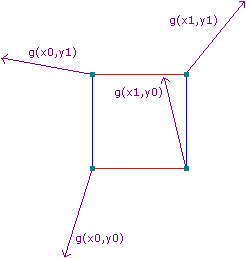
\includegraphics[scale=0.5]{gradients.png}
	\caption{Random Gradients}
	\label{fig:randomGradients}
\end{figure}
\begin{figure}
	\center
	\subfigure{
		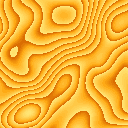
\includegraphics[scale=0.5]{woodgrain.png}
	}
	\subfigure{
		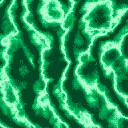
\includegraphics[scale=0.5]{marble.png}
	}
	\subfigure{
		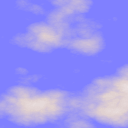
\includegraphics[scale=0.5]{clouds.png}
	}
	\caption{Perlin Noise Examples}
	\label{fig:perlinEg}
\end{figure}
\subsubsection{Simplex Noise}
\subsubsection{Diamond Square}
% subsection algorithms (end)